\subsubsection{Illustrations}
The following sections provide two examples of how ForeC programs
execute. The executions are given as sequences of rewrites.

\subsubsection{Example One}
The first program illustrates parallel execution using
the \verb$par$ statement. Figure~\ref{fig:forec_semantics:program1}
presents the ForeC program, and Figure~\ref{fig:forec_semantics:program1_cfg}
illustrates the program's control-flow. 
In Figure~\ref{fig:forec_semantics:program1_cfg}, the triangle 
represents the forking of threads while the inverted triangle
represents the joining of threads. 

In the program's first 
tick, the parent thread \verb$main$ begins its local tick by
forking two child threads, \verb$t1$ and \verb$t2$. The child
threads start their local ticks by copying the shared variable
\verb$s$. Thread \verb$t1$ pauses while thread \verb$t2$ 
assigns $4$ to its local copy of \verb$s$ and terminates. The 
first tick ends and the shared variable \verb$s$ is resynchronized.
Using the combine policy \verb$all$, the new value (or the 
resynchronized value) of \verb$s$
becomes \verb$plus$$(0,4) = 4$.
In the second tick, thread~\verb$t1$ starts
its local tick by creating a copy of \verb$s$, assigning
$3$ to its copy of \verb$s$, and then terminating. The 
\verb$par$ terminates because threads \verb$t1$ and 
\verb$t2$ have now joined. Because only thread \verb$t1$ 
has a copy of \verb$s$, that copy is assigned directly to 
its parent thread \verb$main$. The \verb$main$ thread starts
its local tick which results in the program terminating.
The second tick ends and the shared variable~\verb$s$ is 
resynchronized with the value $3$
because only the \verb$main$ thread has a copy of \verb$s$.

\begin{figure}
	\centering

	\hfill
	\begin{minipage}{0.47\columnwidth}
		\subfloat[ForeC program.] {
			\lstinputlisting[style=full]{./code/forec/illustration/program1.forec}
			\label{fig:forec_semantics:program1}
		}

		\subfloat[Translated kernel program.] {
			\lstinputlisting[style=full]{./code/forec/illustration/program1_kernel.forec}
			\label{fig:forec_semantics:program1_kernel}
		}
	\end{minipage}
	\begin{minipage}{0.4\columnwidth}
		\subfloat[Control-flow graph.] {
			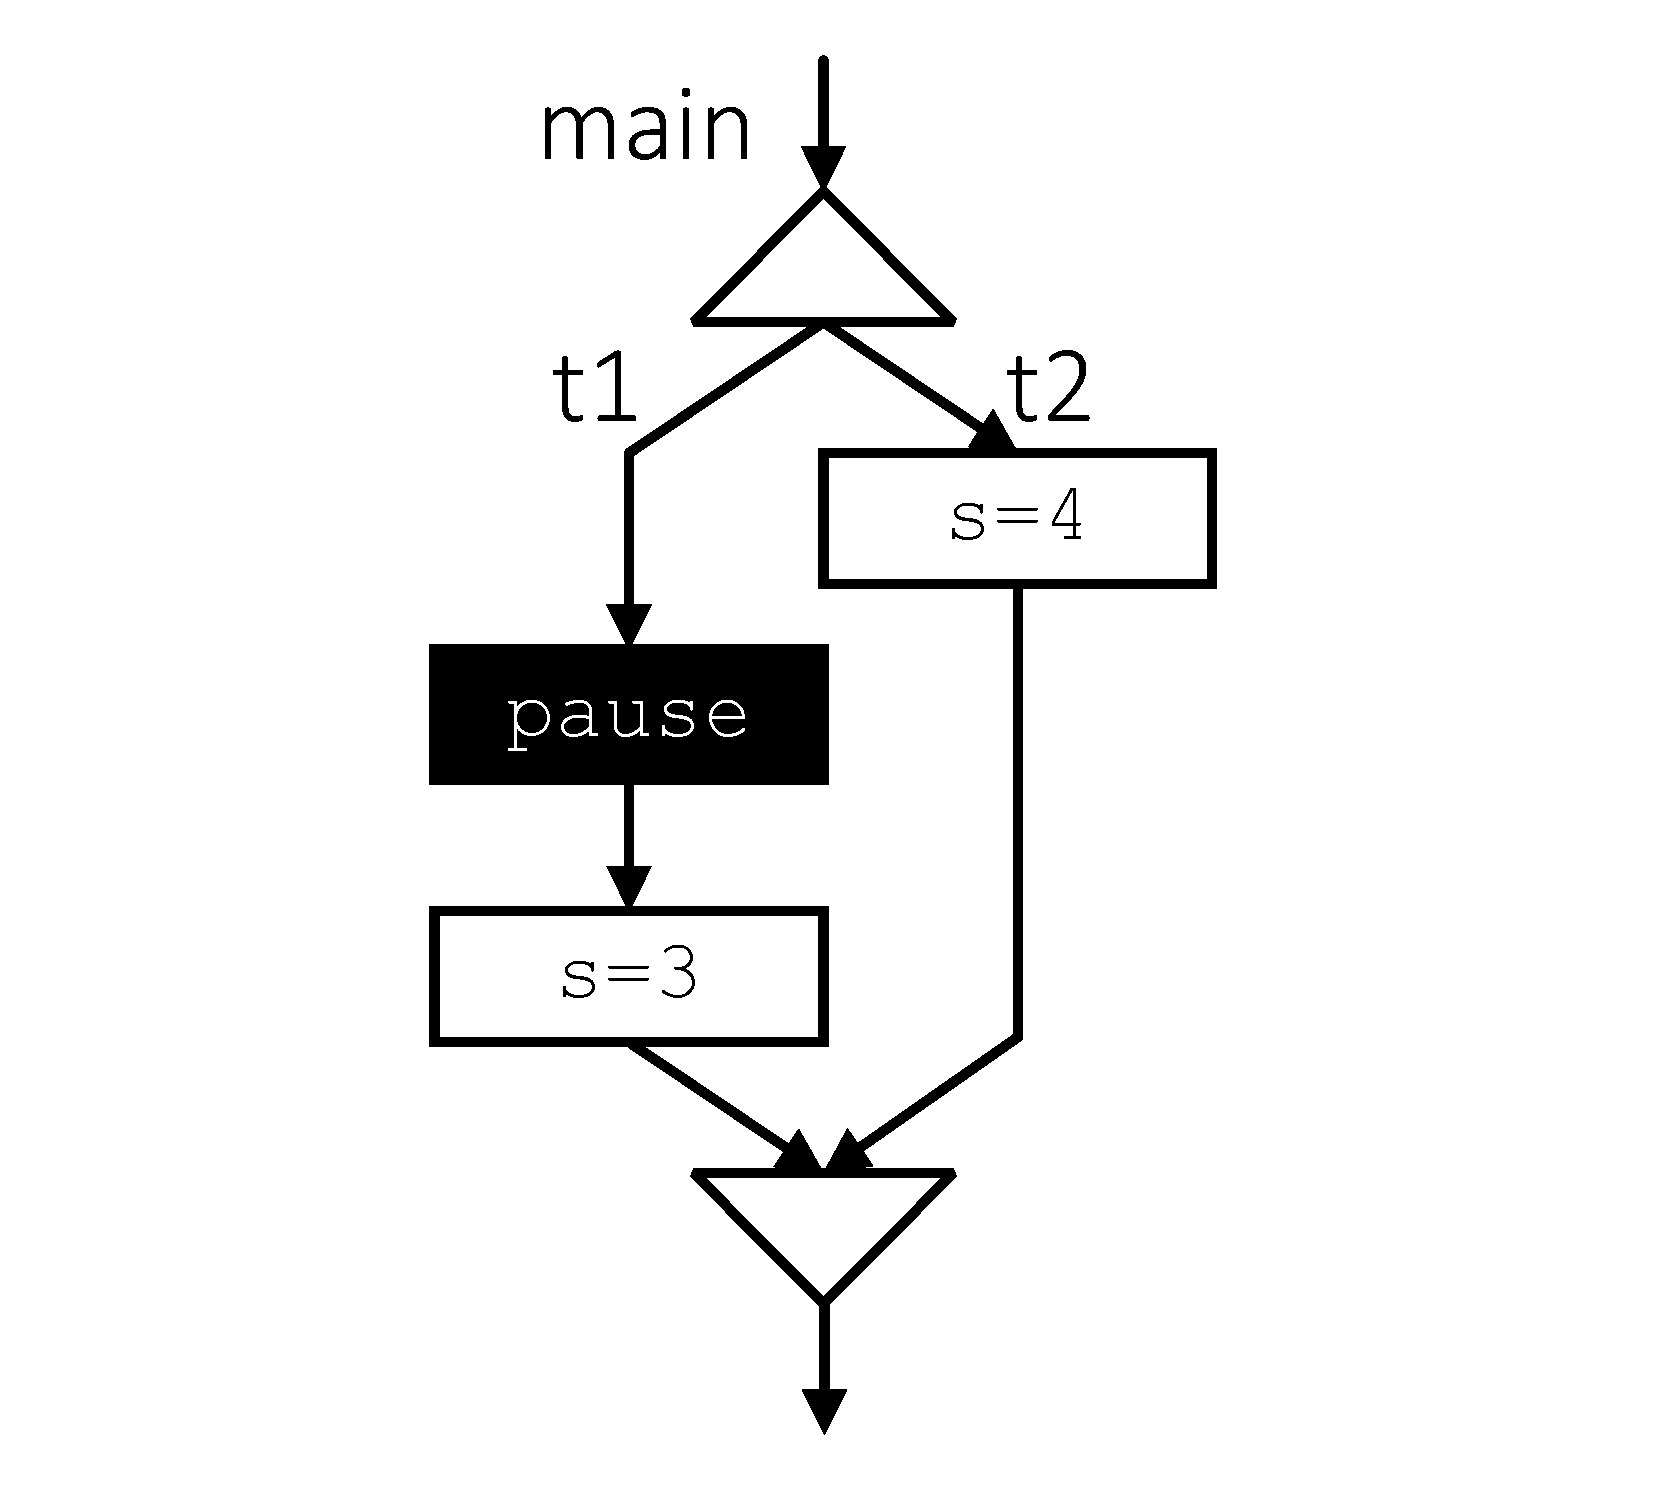
\includegraphics[width=\columnwidth]{program1_cfg}
			\label{fig:forec_semantics:program1_cfg}
		}
	\end{minipage}
	\hspace{0.1cm}

	\caption{Illustrative example one.}
\end{figure}

Before we apply the rewrite rules to the program, 
it is structurally translated into 
Figure~\ref{fig:forec_semantics:program1_kernel} 
(see the start of Section~\ref{sec:forec_semantics}).
Note that the semantic functions $\GetShared($\verb$main$$)$, 
$\GetShared($\verb$t1$$)$, $\GetShared($\verb$t2$$)$ 
and $\GetShared(\Global)$ all return $\lbrace$\verb$s$$\rbrace$.
The set of preemption statuses \Abort{} is initially $\emptyset$.
The program's environment \Environment{} and its derivatives 
are defined in Figure~\ref{figure:forec_program_2}.
\newline

\begin{figure}
	\centering
	$$\begin{array}{l l l}
		\Environment		&=& \left \lbrace
									\Global \to \lbrace s \to (0, \texttt{pre}) \rbrace
								\right \rbrace		\\
		\Environment^1		&=& \left \lbrace
									\Global \to \lbrace s \to (0, \texttt{pre}) \rbrace,
									main \to \lbrace s \to (0, \texttt{pre}) \rbrace
								\right \rbrace		\\
		\Environment^2		&=& \left \lbrace
									\Global \to \lbrace s \to (0, \texttt{pre}) \rbrace,
									main \to \lbrace s \to (0, \texttt{pre}) \rbrace,
									t1 \to \lbrace s \to (0, \texttt{pre}) \rbrace
								\right \rbrace		\\
		\Environment^3		&=& \left \lbrace
									\Global \to \lbrace s \to (0, \texttt{pre}) \rbrace,
									main \to \lbrace s \to (0, \texttt{pre}) \rbrace,
									t2 \to \lbrace s \to (0, \texttt{pre}) \rbrace
								\right \rbrace		\\
		\Environment^4		&=& \left \lbrace
									\Global \to \lbrace s \to (0, \texttt{pre}) \rbrace,
									main \to \lbrace s \to (0, \texttt{pre}) \rbrace,
									t1 \to \lbrace s \to (0, \texttt{pre}) \rbrace,
									t2 \to \lbrace s \to (0, \texttt{pre}) \rbrace
								\right \rbrace		\\
		\Environment^5		&=& \left \lbrace
									\Global \to \lbrace s \to (0, \texttt{pre}) \rbrace,
									main \to \lbrace s \to (0, \texttt{pre}) \rbrace,
									t1 \to \lbrace s \to (0, \texttt{pre}) \rbrace,
									t2 \to \lbrace s \to (4, \texttt{mod}) \rbrace
								\right \rbrace		\\
		\Environment^6		&=& \left \lbrace
									\Global \to \lbrace s \to (0, \texttt{pre}) \rbrace,
									main \to \lbrace s \to (4, \texttt{cmb}) \rbrace
								\right \rbrace		\\
		\Environment^7		&=& \left \lbrace
									\Global \to \lbrace s \to (4, \texttt{pre}) \rbrace
								\right \rbrace		\\
		\\
		\Environment^8		&=& \left \lbrace
									\Global \to \lbrace s \to (4, \texttt{pre}) \rbrace,
									t1 \to \lbrace s \to (4, \texttt{pre}) \rbrace
								\right \rbrace		\\
		\Environment^9		&=& \left \lbrace
									\Global \to \lbrace s \to (4, \texttt{pre}) \rbrace,
									t1 \to \lbrace s \to (3, \texttt{mod}) \rbrace
								\right \rbrace		\\
		\Environment^{10}	&=& \left \lbrace
									\Global \to \lbrace s \to (4, \texttt{pre}) \rbrace,
									main \to \lbrace s \to (3, \texttt{cmb}) \rbrace
								\right \rbrace		\\
		\Environment^{11}	&=& \left \lbrace
									\Global \to \lbrace s \to (3, \texttt{pre}) \rbrace
								\right \rbrace
	\end{array}$$
	
	\caption{Initial program environment and its derivatives.}
	\label{figure:forec_program_2}
\end{figure}

\noindent
\textbf{Step 1:}
Start the tick by applying the (\ref{forec:seq-right}) and
(\ref{forec:copy}) rules. 
\begin{prooftree}
			\AxiomC{}
		\LeftLabel{(\ref{forec:copy})}
		\UnaryInfC{$\langle \Environment, \Abort \rangle ~ \texttt{main:copy}
						\xrightarrow[~~\Input~~]{0} 
					\langle \Environment^1, \Abort \rangle ~ \texttt{main:}$}
	\LeftLabel{(\ref{forec:seq-right})}
	\UnaryInfC{$\begin{array}{l}
					\langle \Environment, \Abort \rangle ~ \texttt{main:copy;par(t1:\{copy;}	\\
					\texttt{pause;s=3;\},t2:\{copy;s=4;\})}
				\end{array}
					\xrightarrow[~~\Input~~]{\bot} 
				\begin{array}{l}
					\langle \Environment^1, \Abort \rangle ~ \texttt{main:par(t1:\{copy;}			\\
					\texttt{pause;s=3;\},t2:\{copy;s=4;\})}
				\end{array}$}
\end{prooftree}

\noindent
\textbf{Step 2:}
Both threads of the \texttt{par} execute sequential statements.
Apply the (\ref{forec:par-1}) rule. Additionally, apply the
(\ref{forec:seq-right}) and (\ref{forec:copy}) rules to both
threads. The environments of both threads, $\Environment^2$
and $\Environment^3$, are aggregated into $\Environment^4$.
\begin{prooftree}
				\AxiomC{}
			\LeftLabel{(\ref{forec:copy})}
			\UnaryInfC{$\langle \Environment^1, \Abort \rangle ~ \texttt{t1:copy}
							\xrightarrow[~~\Input~~]{0} 
						\langle \Environment^2, \Abort \rangle ~ \texttt{t1:}$}
		\LeftLabel{(\ref{forec:seq-right})}
		\UnaryInfC{$\begin{array}{l}
						\langle \Environment^1, \Abort \rangle ~ \texttt{t1:copy;}			\\
						\texttt{pause;s=3}
					\end{array}
						\xrightarrow[~~\Input~~]{\bot} 
					\begin{array}{l}
						\langle \Environment^2, \Abort \rangle ~ \texttt{t1:}				\\
						\texttt{pause;s=3}
					\end{array}$}
		%
				\AxiomC{}
			\UnaryInfC{$\langle \Environment^1, \Abort \rangle ~ \texttt{t2:copy}
							\xrightarrow[~~\Input~~]{0} 
						\langle \Environment^3, \Abort \rangle ~ \texttt{t2:}$}
		\UnaryInfC{$\begin{array}{l}
						\langle \Environment^1, \Abort \rangle ~ \texttt{t2:}					\\
						\texttt{copy;s=4;}
					\end{array}
						\xrightarrow[~~\Input~~]{\bot}
					\begin{array}{l}
						\langle \Environment^3, \Abort \rangle ~ \texttt{t2:}				\\
						\texttt{~~~~~~~s=4;}
					\end{array}$}
	%	
	\LeftLabel{(\ref{forec:par-1})}
	\BinaryInfC{$\begin{array}{l}
					\langle \Environment^1, \Abort \rangle ~ \texttt{main:par(t1:\{copy;}		\\
					\texttt{pause;s=3;\},t2:\{copy;s=4;\})}
				\end{array}
					\xrightarrow[~~\Input~~]{\bot} 
				\begin{array}{l}
					\langle \Environment^4, \Abort \rangle ~ \texttt{main:par(t1:\{pause;}		\\
					\texttt{~~~~~~~s=3;\},t2:\{s=4;\})}
				\end{array}$}
\end{prooftree}

\noindent
\textbf{Step 3:}
Apply the (\ref{forec:tick}) and (\ref{forec:par-7}) rules.
Additionally, apply the (\ref{forec:seq-left}) and
(\ref{forec:pause}) rules to the first thread and the
(\ref{forec:assign-shared}) rule to the second thread.
\textbf{The program completes the tick.} Note that when the
(\ref{forec:par-7}) rule is applied, the aggregated
environment is the same as~$\Environment^5$, which is then
combined to be $\Environment^6$. When the (\ref{forec:tick})
rule is applied, $\Environment^6$ is resynchronized to be
$\Environment^7$.
\begin{prooftree}
					\AxiomC{}
				\LeftLabel{(\ref{forec:pause})}
				\UnaryInfC{$\begin{array}{l}
								\langle \Environment^4, \Abort \rangle ~ \texttt{t1:}		\\
								\texttt{~~~~pause}
							\end{array}
								\xrightarrow[~~\Input~~]{1}
							\begin{array}{l}
								\langle \Environment^4, \Abort \rangle ~ \texttt{t1:}		\\
								\texttt{~~~~~copy}
							\end{array}$}
			\LeftLabel{(\ref{forec:seq-left})}
			\UnaryInfC{$\begin{array}{l}
							\langle \Environment^4, \Abort \rangle ~ \texttt{t1:}			\\
							\texttt{pause;s=3}
						\end{array}
							\xrightarrow[~~\Input~~]{1}
						\begin{array}{l}
							\langle \Environment^4, \Abort \rangle ~ \texttt{t1:}			\\
							\texttt{copy;s=3}
						\end{array}$}
			%
				\AxiomC{$s \in \lbrace s \rbrace$}
			\LeftLabel{(\ref{forec:assign-shared})}
			\UnaryInfC{$\begin{array}{l}
							\langle \Environment^4, \Abort \rangle ~ \texttt{t2:}			\\
							\texttt{~~~~~~s=4;}
						\end{array}
							\xrightarrow[~~\Input~~]{0} 
						\langle \Environment^5, \Abort \rangle ~ \texttt{t2:}$}
		%
		\LeftLabel{(\ref{forec:par-7})}
		\BinaryInfC{$\begin{array}{l}
						\langle \Environment^4, \Abort \rangle ~ \texttt{main:par(t1:\{pause;}	\\
						\texttt{~~~~~~~s=3;\},t2:\{s=4;\})}
					\end{array}
						\xrightarrow[~~\Input~~]{1} 
					\begin{array}{l}
						\langle \Environment^6, \Abort \rangle ~ \texttt{main:par(t1:\{copy;}	\\
						\texttt{~~~~~~~s=3;\},t2:nop)}
					\end{array}$}
	\LeftLabel{(\ref{forec:tick})}
	\UnaryInfC{$\begin{array}{l}
					\langle \Environment^4, \Abort \rangle ~ \texttt{main:par(t1:\{pause;}		\\
					\texttt{~~~~~~~s=3;\},t2:\{s=4;\})}
				\end{array}
					\xrightarrow[~~\Input~~]{1} 
				\begin{array}{l}
					\langle \Environment^7, \Abort \rangle ~ \texttt{main:par(t1:\{copy;}		\\
					\texttt{~~~~~~~s=3;\},t2:nop)}
				\end{array}$}
\end{prooftree}

\noindent
\textbf{Step 4:}
Start the next tick by applying the (\ref{forec:par-3})
rule. Additionally, apply the (\ref{forec:seq-right}) and
(\ref{forec:copy}) rules to the first thread and the
(\ref{forec:nop}) rule to the second thread.
\begin{prooftree}
				\AxiomC{}
			\LeftLabel{(\ref{forec:copy})}
			\UnaryInfC{$\langle \Environment^7, \Abort \rangle ~ \texttt{t1:copy}
							\xrightarrow[~~\Input~~]{0} 
						\langle \Environment^8, \Abort \rangle ~ \texttt{t1:}$}
		\LeftLabel{(\ref{forec:seq-right})}
		\UnaryInfC{$\begin{array}{l}
						\langle \Environment^7, \Abort \rangle ~ \texttt{t1:}				\\
						\texttt{copy;s=3}
					\end{array}
						\xrightarrow[~~\Input~~]{\bot}
					\langle \Environment^8, \Abort \rangle ~ \texttt{t1:s=3}$}
		%
			\AxiomC{}
		\LeftLabel{(\ref{forec:nop})}
		\UnaryInfC{$\begin{array}{l}
						\langle \Environment^7, \Abort \rangle ~ \texttt{t2:}				\\
						\texttt{~~~~~~~nop}
					\end{array}
						\xrightarrow[~~\Input~~]{0} 
					\langle \Environment^7, \Abort \rangle ~ \texttt{t2:}$}
	%
	\LeftLabel{(\ref{forec:par-3})}
	\BinaryInfC{$\begin{array}{l}
					\langle \Environment^7, \Abort \rangle ~ \texttt{main:par(t1:\{copy;}	\\
					\texttt{~~~~~~~s=3;\},t2:nop)}
				\end{array}
					\xrightarrow[~~\Input~~]{\bot} 
				\langle \Environment^8, \Abort \rangle ~ \texttt{main:par(t1:\{s=3;\},t2:nop)}$}
\end{prooftree}

\noindent
\textbf{Step 5:}
Apply the (\ref{forec:par-5}) rule. Additionally, apply the
(\ref{forec:assign-shared}) rule to the first thread and the
(\ref{forec:nop}) rule to the second thread. Note that when
the (\ref{forec:par-5}) rule is applied, the aggregated
environment is the same as $\Environment^9$, which is then
combined to be~$\Environment^{10}$.
\begin{prooftree}
			\AxiomC{$s \in \lbrace s \rbrace$}
		\LeftLabel{(\ref{forec:assign-shared})}
		\UnaryInfC{$\begin{array}{l}
						\langle \Environment^8, \Abort \rangle ~ \texttt{t1:}				\\
						\texttt{~~~~~~s=3}
					\end{array}
						\xrightarrow[~~\Input~~]{0} 
					\langle \Environment^9, \Abort \rangle ~ \texttt{t1:}$}
	%
			\AxiomC{}
		\LeftLabel{(\ref{forec:nop})}
		\UnaryInfC{$\begin{array}{l}
						\langle \Environment^8, \Abort \rangle ~ \texttt{t2:}				\\
						\texttt{~~~~~~nop}
					\end{array}
						\xrightarrow[~~\Input~~]{0} 
					\langle \Environment^8, \Abort \rangle ~ \texttt{t2:}$}
	%
	\LeftLabel{(\ref{forec:par-5})}
	\BinaryInfC{$\langle \Environment^8, \Abort \rangle ~ \texttt{main:par(t1:\{s=3;\},t2:nop)}
					\xrightarrow[~~\Input~~]{\bot} 
				\langle \Environment^{10}, \Abort \rangle ~ \texttt{main:copy}$}
\end{prooftree}

\noindent
\textbf{Step 6:}
Apply the (\ref{forec:tick}) and (\ref{forec:copy}) rules.
The environment $\Environment^{10}$ is resynchronized to be
$\Environment^{11}$. \textbf{The tick ends and the program terminates.}
\begin{prooftree}
			\AxiomC{}
		\LeftLabel{(\ref{forec:copy})}
		\UnaryInfC{$\langle \Environment^{10}, \Abort \rangle ~ \texttt{main:copy}
						\xrightarrow[~~\Input~~]{0} 
					\langle \Environment^{10}, \Abort \rangle ~ \texttt{main:}$}
	\LeftLabel{(\ref{forec:tick})}
	\UnaryInfC{$\langle \Environment^{10}, \Abort \rangle ~ \texttt{main:copy}
					\xrightarrow[~~\Input~~]{0} 
				\langle \Environment^{11}, \Abort \rangle ~ \texttt{main:}$}
\end{prooftree}
